% !TeX root = ../paper_observer_consciousness.tex

\begin{wrapfigure}{r}{0.4\textwidth}
	\centering
	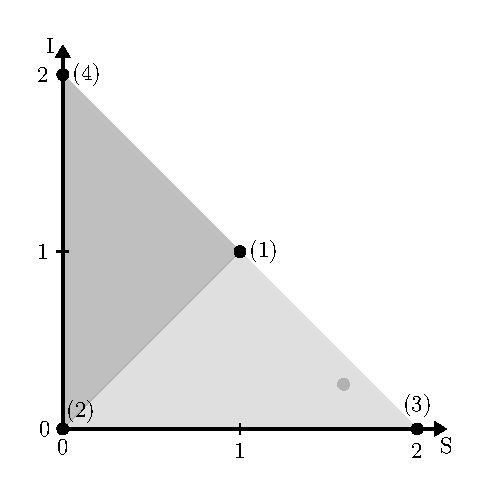
\includegraphics[scale=0.8]{graphics/presentation_qm_extra.pdf}
	\caption{Darstellung der Transinformation $I$ eines 2-bit/2-qbit-Systems in Abhängigkeit seiner
		Entropie $S$. Klassische Systeme können nur in dem hellen Dreieck liegen, während quantenmechanisch
		zusätzlich das dunklen Dreieck möglich ist. Markiert sind die 4 Zustände:
		(1): $\rho = \frac{1}{2} \del{\ketup\!\braup + \ketdown\!\bradown}$, (2): $\rho = \ketup\!\braup$,
		(3): $\rho = \frac{1}{4} (\ketup\!\braup + \ketdown\!\braup+ \ketup\!\bradown + \ketdown\!\bradown)$,
		(4): $\rho = \frac{1}{2} \del{\ketup\!\ketup + \ketdown\!\ketdown}$. Der hell graue Punkt stellt für dieses 
		2-qbit-System die maximal mögliche Integrierte Information dar. \label{fig:independence_plot}}
\end{wrapfigure}  

Wie im vorherigen Abschnitt gesehen, führt maximale Integration zu einer so komplexen Dynamik,
dass diese im menschlichen Gehirn nicht realisiert sein kann. Im Folgenden soll nun  
betrachtet werden wie groß die Unabhängigkeit zwischen Teilsystemen werden kann und welche Konsequenzen
aus dieser Unabhängigkeit resultieren. Als Maß kann dabei wiederum die Integrierte Information dienen, für maximal 
unabhängige Teilsysteme hat diese den Wert $\Phi = 0$.

Bei der Betrachtung von Unabhängigkeit stellt man eine großen Unterschied zwischen klassischen und 
quantenmechanischen Systemen fest. Zur Verdeutlichung sollen hier ein klassisches 2-bit- und ein quantenmechanisches
2-qbit-System betrachtet werde. Die Zustände, die von diesen beiden Systemen eingenommen werden 
können alle als Punkt in dem Koordinatensystem aus $(S,I)$ in \cref{fig:independence_plot} eingetragen werden.
Dabei ist das klassische System auf das helle Dreieck beschränkt, während das 2-qbit-System zusätzlich im dunklen 
Dreieck liegen kann.



Die Berechnung der Integrierten Information des klassischen Systems erweist sich als trivial, da nur ein 
einziger Schnitt in zwei Teilsysteme (jeweils ein bit) möglich ist und somit $\Phi = I$ gilt.
Für das Quantensystem ergibt sich jedoch das Problem, dass jede Basis des Hilbertraums gleich bedeutend
ist und daher die Minimierung der Transinformation kontinuierlich über alle unitären Transformationen 
durch geführt werden muss.
\begin{empheq}{equation}
	\Phi = \displaystyle\min_{U} I\del{U\rho U^{\dagger}}
\end{empheq}  
Dies führt dazu das selbst der Zustand (4) in \cref{fig:independence_plot}, einer der vier maximal verschränkten 
Bell-Zustände, in einen reinen Zustand transformiert werden kann, sodass für diesen $\Phi= 0$ gilt.
Die für Quantenzustände maximal mögliche Integrierte Information kann für ein System der betrachteten
Größe zu $\Phi = \num{0.2516}$ bit bestimmt werden. Dieser Wert ist als grauer Punkt in \cref{fig:independence_plot} 
eingezeichnet. Und auch für größere System zeigt sich, dass
$\Phi$ für klassische Systeme annähernd linear mit der Systemgröße steigt während $\Phi$ für Quantensystem 
gegen null geht. Damit zeigt sich das Zustände von Quantensystemen im Vergleich zu klassischen Zuständen wesentlich 
unabhängiger sind.

Betrachtet man wiederum die Integrierte Information des gesamten Systems, beschrieben durch $H$, 
der allgemein in drei Teile separiert werden kann
\begin{empheq}{equation}
	H = H_{1} \otimes I  +  I \otimes H_{2} + H_{3}
\end{empheq}
so ist leicht zu verstehen, dass diese am geringsten ist, wenn der Wechselwirkungsterm $H_3$ minimal wird.
Wird eine solche Separation gefunden gilt, da $H_1$ und $H_2$ näherungsweise unabhängig sind, dass 
$\comm{H_i}{H_j} = 0$ und $\comm{H_i}{H_3} = 0$ für $i,j \in {1,2}$. Das Vertauschen des System Hamiltonoperators
mit dem Wechselwirkungsterm führt nun aber dazu, dass Zustände durch die Dekohärenz in einen zeitunabhängigen
Zustand getrieben werden. Trennt man das Universum also in möglichst unabhängige Teile auf, so kommt jegliche 
Veränderung zum erliegen.     


